\Section{Theoretical Foundations}
\label{ch:theory}

\Subsection{The Standard Model of Particle Physics}

The Standard Model of Particle Physics (Standard Model or SM) is our best understanding of the fundamental interactions (strong, weak and the electromagnetic interaction, excluding gravity due to the inaccessibility of the scales it acts under laboratory conditions) occurring in nature. It describes the dynamics of elementary particles and the processes they undergo upon production or decay.

These elementary particles can be sorted into quarks, leptons and interaction carrier particles. Quarks take part in the strong interaction and couple directly to its mediator particles, the gluons. Leptons on the other hand are left invariant by them. These particles can be sorted into isospin tuples and into three generations and they can be electrically charged or neutral. In the former case, they couple to photons and hence participate in the electromagnetic interaction. The $Z$ and $W$ bosons are the mediators of the weak interaction. The newest addition to this family, the Higgs-boson is responsible for generating the masses of the electroweak force-carriers and of the quarks and leptons.

Regarding their spin, one distinguishes between two main categories: bosons (particles of integer spin) and fermions (particles with half-odd integer spin). All quarks and leptons are fermions and all force carriers are of bosonic nature. Fig. \ref{fig:sm} shows an overview of all elementary particles grouped along the above-mentioned criteria.


The SM Lagrangian can be written in a compact and elegant form as

%\begin{align}
%	\begin{split}
%		\mathcal{L} = &-\frac{1}{4}F_{\mu\nu}F^{\mu\nu} \\ &+ i \bar{\psi}\slashed{D}\psi \\ &+ \psi_iy_{ij}\psi_j\phi + h.c. \\ &+ |D_\mu\phi|^2 - V(\phi)
%	\end{split}
%	\label{eq:lagrangian}
%\end{align}

\begin{equation}
		\mathcal{L} = \underbrace{-\frac{1}{4}F_{\mu\nu}F^{\mu\nu}}_{\mathcal{L}_g} + \underbrace{\vphantom{-\frac{1}{4}F_{\mu\nu}F^{\mu\nu}}i \bar{\psi}\slashed{D}\psi}_{\mathcal{L}_f} + \underbrace{\vphantom{-\frac{1}{4}F_{\mu\nu}F^{\mu\nu}}\psi_iy_{ij}\psi_j\phi + h.c.}_{\mathcal{L}_\text{Yuk}} + \underbrace{\vphantom{-\frac{1}{4}F_{\mu\nu}F^{\mu\nu}}|D_\mu\phi|^2 - V(\phi)}_{\mathcal{L}_H}
	\label{eq:lagrangian}
\end{equation}

The first term $\mathcal{L}_g$ describes the interaction of the gauge bosons among each other; the second term $\mathcal{L}_f$ encodes the interaction between fermions altogether. The $\mathcal{L}_\text{Yuk}$ term contains the Yukawa-couplings of the fermions to the Higgs field. The final and fourth term $\mathcal{L}_H$ describes the interplay between the Higgs and the gauge bosons and the Higgs field itself through the potential $V(\phi)$

\begin{figure}[h!]
	\centering
	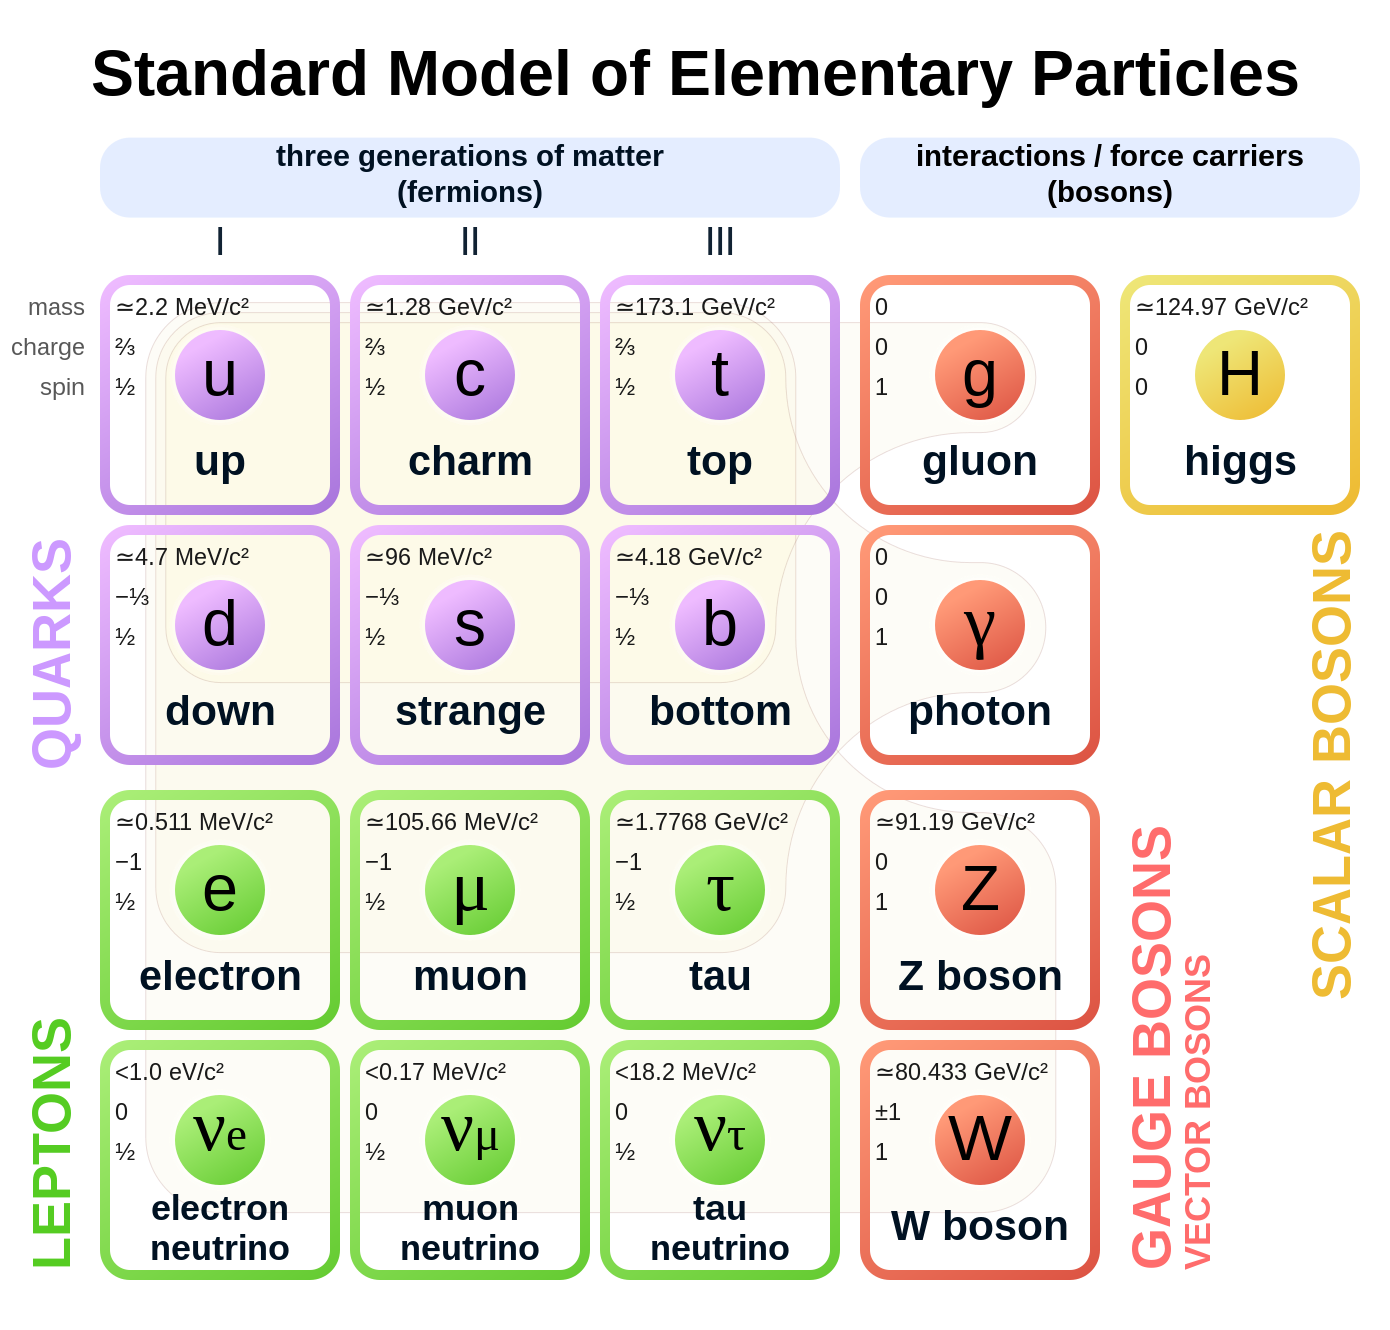
\includegraphics[width=0.6\linewidth]{figures/theory/sm.png}
	\caption{The Standard Model of Elementary Particles. Note the three generation of quarks and leptons, and their isospin doublet scheme. The four force carriers and the Higgs boson are listed on right. \cite{enwiki:1101993746}}
	\label{fig:sm}
\end{figure}

Despite its incredible predictivity, it is known that the Standard Model is an incomplete description of nature. For this reason, several SM testing precision and BSM measurements are performed.

\Subsection{The Higgs Mechanism and the Higgs Boson}
The Higgs term in the Lagragian from eq. \ref{eq:lagrangian} gives rise to the mass of the gauge bosons. The potential $V(\phi)$ is given by

\begin{equation*}
	V(\phi) = -\mu^2 \phi^\dagger \phi + \frac{\lambda}{4}\left(\phi^\dagger\phi\right)^2 
\end{equation*}

and is rotational symmetric and takes a "Mexican hat"-like shape. The form of the potential in the complex plane is shown if fig. \ref{fig:mexicanhat}.

\begin{figure}[h!]
	\centering
	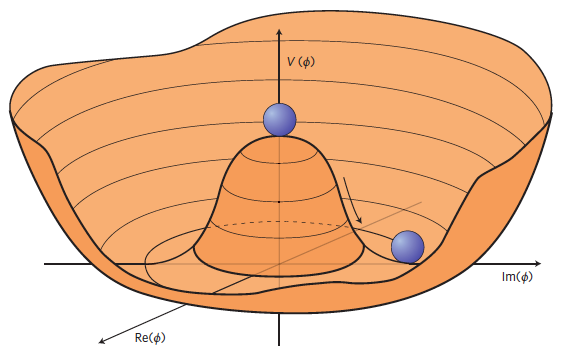
\includegraphics[width=0.8\linewidth]{figures/theory/higgspotential}
	\caption{Shape of the Higgs potential ("Mexican hat"). Note the location of the field minimum at $\phi \neq 0$, resulting in the Higgs field obtaining a vacuum expectation value. \cite{Ellis:2012465}}
	\label{fig:mexicanhat}
\end{figure}

Due to the location of the potential minimum lying at $\phi \neq 0$ the field $\phi$ obtains a vacuum expectation value (spontaneous symmetry breaking). In addition to that, due to the covariant derivative $D_\mu$, additional coupling terms of the gauge bosons to this field $\phi$ appear. It turns out, that by writing the field $\phi$ as

\begin{equation*}
	\phi = \frac{1}{\sqrt{2}}\left(\begin{matrix}
		0 \\
		v + H
	\end{matrix}
	\right)
\end{equation*}

where $v$ is the location of the potential minimum (a constant) and $H$ is real scalar field, the electroweak gauge bosons  obtain a mass through the constant $v$

\begin{equation*}
	m^2_W = \frac{g^2 v^2}{4}, \quad m^2_Z = \frac{(g'^2 + g^2)v^2}{4}
\end{equation*}

with the electroweak coupling constants $g$, and $g'$. Not only the gauge bosons obtain a mass thanks to the Higgs field though. Through the Yukawa coupling, fermions (and all massive particles at tree level) couple directly to the Higgs boson with a coupling dependent on their mass and spin. Additionally, the resulting Lagrangian density respects the physical symmetries

\begin{equation*}
	SU(3)_c \times SU(2)_L \times U(1)_Y
\end{equation*}

which would not have been the case in the absence of the field $\phi$ due to the mass terms of the electroweak gauge bosons. These symmetries of the Lagrangian are responsible for the generation of the colour and electric charges, the latter of which becomes only visible through the spontaneous breaking of the $SU(3)_c \times SU(2)_L \times U(1)_Y$ symmetry into

\begin{equation*}
	SU(3)_c \times U(1)_\text{em}
\end{equation*}

Since its observation in 2012 by the ATLAS and CMS experiments at CERN \cite{Chatrchyan_2012} the properties of the Higgs boson have been extensively studied in detail. The SM Higgs is a CP-even scalar of charge 0 with a measured mass of

\begin{equation*}
	m_H = 125.25 \pm 0.17 \, \text{GeV}
\end{equation*}

The most common Higgs production mechanisms at high energy colliders are shown in fig. \ref{fig:higgsproduction} \cite{Workman:2022ynf}. These are gluon-gluon fusion (ggF), vector-boson fusion (VBF), Higgsstrahlung (VH), associated gauge boson production at one loop from a gluon-gluon interaction, associated top quark pair production ($t\bar{t}H$), and associated single top quark-quark production ($tHq$).

\begin{figure}[h!]
	\centering
	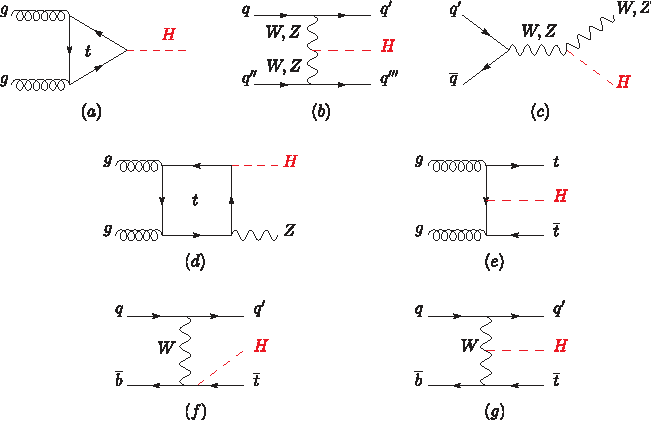
\includegraphics[width=0.8\linewidth]{figures/theory/higgsproduction.pdf}
	\caption{Main Higgs boson production processes in high energy hadron colliders \cite{Workman:2022ynf}. From $(a)$ to $(g)$ these are: ggF $(a)$, VBF $(b)$, Higgs-strahlung $(c)$, associated vector boson production from $gg$ $(d)$, $t\bar{t}H$ $(e)$ and $tHq$ $(f)-(g)$}
	\label{fig:higgsproduction}
\end{figure}

The most common Higgs decay final state branching ratios for various Higgs masses are shown in fig. \ref{fig:higgsbranch}. Note that the main decay channels are swamped with background processes, which made direct detection first available in the $\gamma\gamma$ and $ZZ\rightarrow4l$ final states. Also note that some of the final states are only available through higher-order diagrams as the Higgs couples only to massive particles directly.

\begin{figure}[h!]
	\centering
	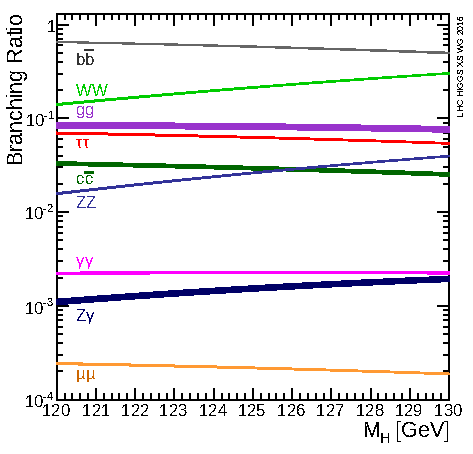
\includegraphics[width=0.6\linewidth]{figures/theory/higgsdecay.pdf}
	\caption{Most common Higgs decay channels expressed as final state branching ratios depending on the Higgs mass. The band widths represent the uncertainties of each channel. \cite{HiggsCrossSections}}
	\label{fig:higgsbranch}
\end{figure}

In the following the gluon-gluon induced vector boson associated Higgs production ($gg\rightarrow VH$) with a focus on a BSM-sensitive physics observable will be discussed in detail.

\Subsection{Gluon-Gluon Induced VH-Higgs Production}

The processes describing $gg\rightarrow VH$ are shown in fig. \ref{fig:VH_diagrams}. As these processes contain loops, they are perfect candidates for SM testing precision measurements. As for the $ZH$ final states of the box and the triangle diagrams interfere destructively, its contribution leads to enhanced sensitivity to BSM physics. This can be seen by the loop itself, to which BSM particles can contribute. Another advantage of the $ZH$ final state is the top-quark exclusive SM contribution which have characteristic thresholds in several kinematic distributions of the cross-section; well-selected cuts increase the number of gluon-initiated events \cite{Harlander_2018}.

\begin{figure}[h!]
	\centering
	\begin{minipage}{.5\textwidth}
		\centering
		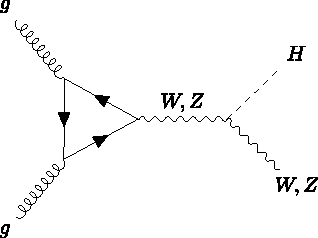
\includegraphics[width=0.8\linewidth]{figures/theory/diagrams/ggVH_triangle.pdf}
	\end{minipage}%
	\begin{minipage}{.5\textwidth}
		\centering
		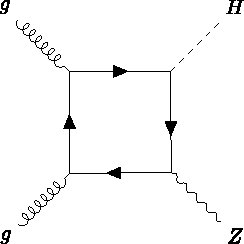
\includegraphics[width=0.6\linewidth]{figures/theory/diagrams/ggZH_box.pdf}
	\end{minipage}
	\caption{Feynman diagrams of the contributing $gg\rightarrow VH$ processes at leading order.}
	\label{fig:VH_diagrams}
\end{figure}

The total cross-section for the VH production can be written as

\begin{equation*}
	\sigma^{VH} = \sigma^{VH}_\text{DY} + \sigma^{VH}_\text{non-DY}
\end{equation*}

where "DY" stands for the contribution of the Drell-Yan-like production channel (the triangle diagram) and non-DY stands for that of the box diagram. Note that in the SM at leading order we can assume that

\begin{equation*}
	\sigma^{WH}_\text{non-DY} = 0.
\end{equation*}

It can be shown, that the ratio $R^{ZH}_\text{DY}$ defined as

\begin{equation}
	R^{ZH}_\text{DY} = \frac{\sigma^{ZH}}{\sigma^{ZH}_\text{DY}} = 1 + \frac{\sigma^{ZH}_\text{non-DY}}{\sigma^{ZH}_\text{DY}}
	\label{eq:ratio}
\end{equation}

is a suitable observable for SM test measurements as it can be seen in fig. \ref{fig:RZH} if one considers the distribution in the invariant $M_{ZH}$ mass.

\begin{figure}[h!]
	\centering
	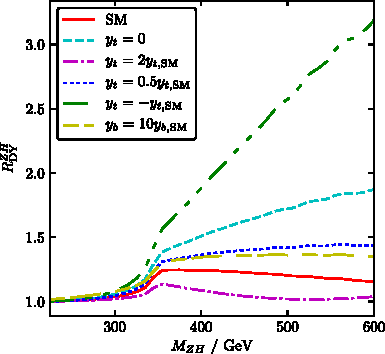
\includegraphics[width=0.6\linewidth]{figures/theory/RZH.pdf}
	\caption{The dependence of the ratio $R^{ZH}_\text{DY}$ on different BSM scenarios in the $M_{ZH}$ distribution. Note that differing top- and bottom quark Yukawa couplings ($y_t$ and $y_b$, respectively), the resulting distribution differs significantly above a threshold of $M_{ZH}=2m_t$, with $m_t$ being the top mass.}
	\label{fig:RZH}
\end{figure}

However, an experiment/theory comparison using $R^{ZH}_\text{DY}$ suffers from arising systematic uncertainties; fortunately it still can be use a basis for other BSM-senstive observables. For this purpose, the similarity between the Drell-Yan-like $WH$ and $ZH$ final states can be exploited. Defining expanded fraction in eq. \ref{eq:ratio} and writing

\begin{equation}
	R^{ZW}_R = \frac{\sigma^{ZH}/\sigma^{WH}}{\sigma^{ZH}_\text{DY}/\sigma^{WH}}
\end{equation}

results in an excellent observable candidate for two reasons. First, it is expected that measuring the nominator $\sigma^{ZH}/\sigma^{WH}$ a number of systematic uncertainties cancel especially if the parameters of $ZH$ and $WH$ analyses are aligned as much as possible. Second, the denominator $\sigma^{ZH}_\text{DY}/\sigma^{WH}$ can be theoretically evaluated with high precision and is insensitive to BSM effects, as the only couplings (the electroweak couplings) in the related processes are experimentally heavily constrained.
